\documentclass[./blockchain.tex

\begin{document}
    \section{Knowledge \& Terms}
    \begin{frame}{Ethereum}{Chain Id, Network Id}
        \begin{itemize}
            \item Network Id and Chain Id are identificators for Ethereum networks
            \item \emph{Network Id} used for peer to peer communication
            \item \emph{Chain Id} is used in transaction signature
            \item For most networks the Chain Id and Network Id are the same.
            \item Genesis block defines the Chain Id

        \end{itemize}


    \end{frame}



    \begin{frame}{Ethereum}{Chain Id, Network Id}

%        Image orgin: https://besu.hyperledger.org/en/stable/Concepts/NetworkID-And-ChainID/

        \begin{figure}
            \centering
            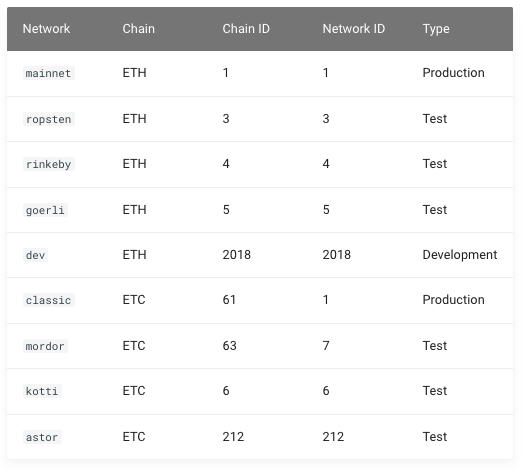
\includegraphics[height=0.7\textheight]{chain-id-network-id}
            \caption{}
            \label{fig:}
        \end{figure}

    \end{frame}

\end{document}




